\documentclass[aspectratio=169]{../latex_main/tntbeamer}  % you can pass all options of the beamer class, e.g., 'handout' or 'aspectratio=43'
\usepackage{dsfont}
\usepackage{bm}
\usepackage[english]{babel}
\usepackage[T1]{fontenc}
%\usepackage[utf8]{inputenc}
\usepackage{graphicx}
\graphicspath{ {./figures/} }
\usepackage{algorithm}
\usepackage[ruled,vlined,algo2e,linesnumbered]{algorithm2e}
\usepackage{hyperref}
\usepackage{booktabs}
\usepackage{mathtools}

\usepackage{amsmath,amssymb}

\DeclareMathOperator*{\argmax}{arg\,max}
\DeclareMathOperator*{\argmin}{arg\,min}

\usepackage{pgfplots}
\pgfplotsset{compat=1.16}
\usepackage{tikz}
\usetikzlibrary{trees} 
\usetikzlibrary{shapes.geometric}
\usetikzlibrary{positioning,shapes,shadows,arrows,calc,mindmap}
\usetikzlibrary{positioning,fadings,through}
\usetikzlibrary{decorations.pathreplacing}
\usetikzlibrary{intersections}
\pgfdeclarelayer{background}
\pgfdeclarelayer{foreground}
\pgfsetlayers{background,main,foreground}
\tikzstyle{activity}=[rectangle, draw=black, rounded corners, text centered, text width=8em]
\tikzstyle{data}=[rectangle, draw=black, text centered, text width=8em]
\tikzstyle{myarrow}=[->, thick, draw=black]

% Define the layers to draw the diagram
\pgfdeclarelayer{background}
\pgfdeclarelayer{foreground}
\pgfsetlayers{background,main,foreground}

% Requires XeLaTeX or LuaLaTeX
\usepackage{unicode-math}

\usepackage{fontspec}
%\setsansfont{Arial}
\setsansfont{RotisSansSerifStd}[ 
Path=../latex_main/fonts/,
Extension = .otf,
UprightFont = *-Regular,  % or *-Light
BoldFont = *-ExtraBold,  % or *-Bold
ItalicFont = *-Italic
]
\setmonofont{Cascadia Mono}[
Scale=0.8
]

% scale factor adapted; mathrm font added (Benjamin Spitschan @TNT, 2021-06-01)
%\setmathfont[Scale=1.05]{Libertinus Math}
%\setmathrm[Scale=1.05]{Libertinus Math}

% other available math fonts are (not exhaustive)
% Latin Modern Math
% XITS Math
% Libertinus Math
% Asana Math
% Fira Math
% TeX Gyre Pagella Math
% TeX Gyre Bonum Math
% TeX Gyre Schola Math
% TeX Gyre Termes Math

% Literature References
\newcommand{\lit}[2]{\href{#2}{\footnotesize\color{black!60}[#1]}}

%%% Beamer Customization
%----------------------------------------------------------------------
% (Don't) Show sections in frame header. Options: 'sections', 'sections light', empty
\setbeamertemplate{headline}{empty}

% Add header logo for normal frames
\setheaderimage{
	% 
\includegraphics[height=\logoheight]{figures/TNT_darkv4.pdf}
	
\includegraphics[height=\logoheight]{../latex_main/figures/luh_logo_rgb_0_80_155.pdf}
	% 
\includegraphics[height=\logoheight]{figures/logo_tntluh.pdf}
}

% Header logo for title page
\settitleheaderimage{
	% 
\includegraphics[height=\logoheight]{figures/TNT_darkv4.pdf}
	
\includegraphics[height=\logoheight]{../latex_main/figures/luh_logo_rgb_0_80_155.pdf}
	% 
\includegraphics[height=\logoheight]{figures/logo_tntluh.pdf}
}

% Title page: tntdefault 
\setbeamertemplate{title page}[tntdefault]  % or luhstyle
% Add optional title image here
%\addtitlepageimagedefault{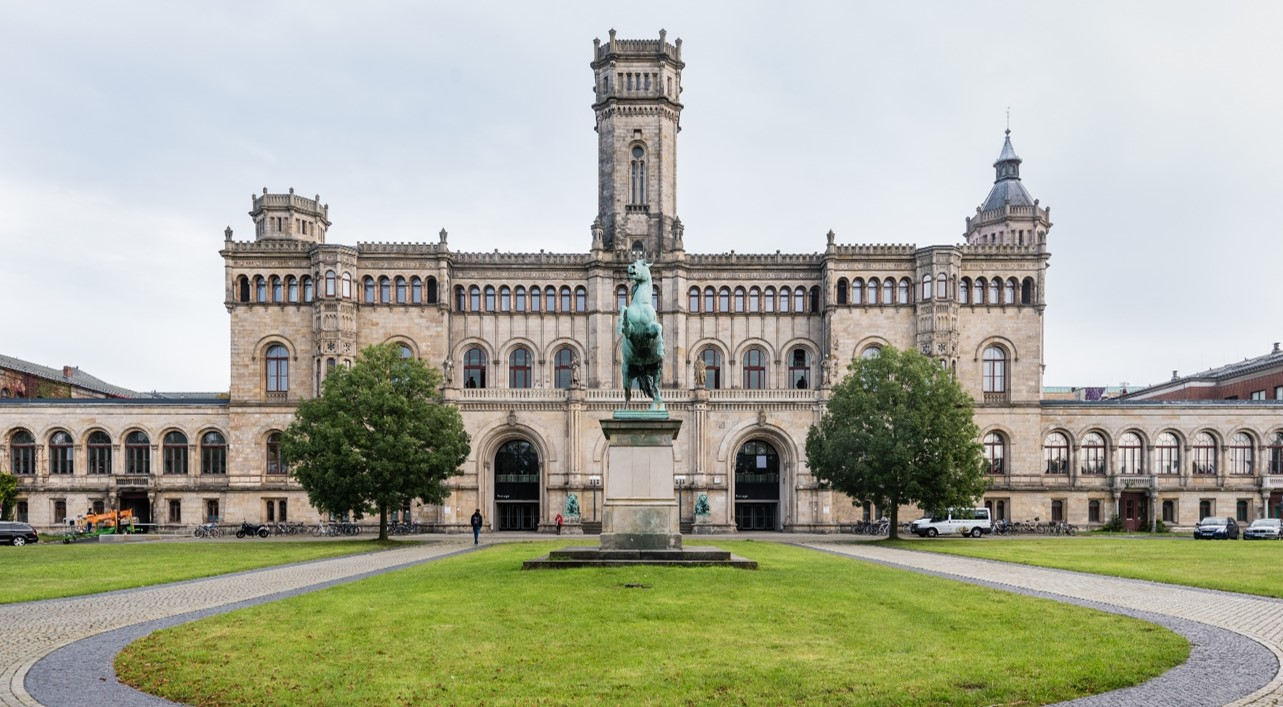
\includegraphics[width=0.65\textwidth]{figures/luh_default_presentation_title_image.jpg}}

% Title page: luhstyle
% \setbeamertemplate{title page}[luhstyle]
% % Add optional title image here
% \addtitlepageimage{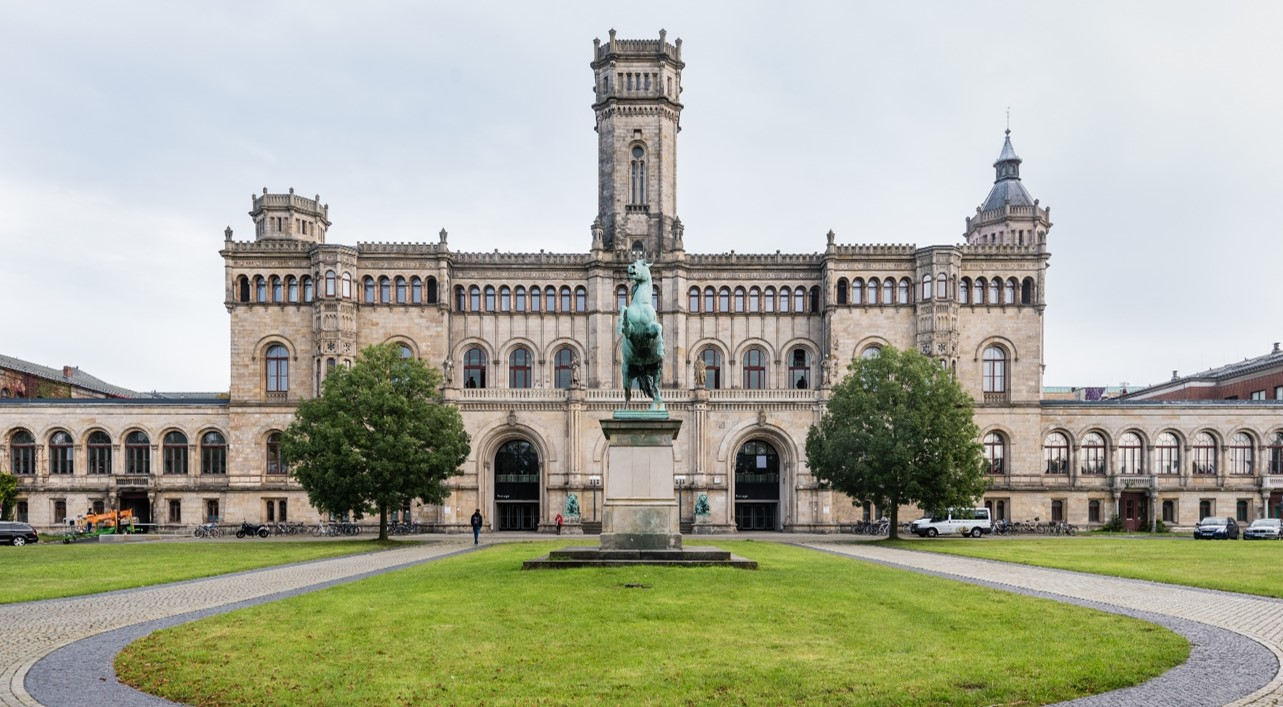
\includegraphics[width=0.75\textwidth]{figures/luh_default_presentation_title_image.jpg}}

\author[Lindauer \& Anand]{Marius Lindauer and Avishek Anand\\[1em]
	
\includegraphics[height=\logoheight]{../latex_main/figures/luh_logo_rgb_0_80_155.pdf}\qquad

\includegraphics[height=\logoheight]{../latex_main/figures/TNT_darkv4}\qquad

\includegraphics[height=\logoheight]{../latex_main/figures/L3S.jpg}	}
\date{Winter Term 2021
}


%%% Custom Packages
%----------------------------------------------------------------------
% Create dummy content
\usepackage{blindtext}

% Adds a frame with the current page layout. Just call \layout inside of a frame.
\usepackage{layout}


\title[Introduction]{iML: Local Explanations}
\subtitle{Examples}

%\institute{}


\begin{document}
	
	\maketitle

	%-----------------------------------------------------------------------------------------------------------------------------

\begin{frame}{Credit Dataset}
    \vspace{-2em}
	\begin{itemize}
		\item We demonstrate local explanation methods on the German credit classification dataset from Kaggle. \href{https://www.kaggle.com/uciml/german-credit}{\beamergotobutton{Click here}}
		\item The dataset has 522 observations and nine features wrt credit and customer information.
		\item The binary target indicates whether a customer has a `good' or `bad' credit risk.  
		\item We combined categories with few case numbers. 
	\end{itemize}
		\begin{center}
			\footnotesize
			\begin{tabular}{ccc}
				\toprule
				name & type & range\\
				\midrule
				age & numeric & [19, 75]\\
				sex & factor & \{male, female\}\\
				job & factor & \{0, 1, 2, 3\}\\
				housing & factor & \{free, own, rent\}\\
				saving.accounts & factor & \{little, moderate, rich\}\\
				checking.accounts & factor & \{little, moderate, rich\}\\
				credit.amount & numeric & [276, 18424]\\
				duration & numeric &  [6, 72]\\
				purpose & numeric &  \{others, car, furniture, radio/TV\}\\
				risk & factor & \{good, bad\}\\
				\bottomrule
			\end{tabular}
		\end{center}
\end{frame}

\begin{frame}{Credit Dataset}

\vspace{-1.5em}
	\begin{itemize}
		\item Model: SVM with RBF kernel
		\item $x$: first data point of the dataset with $\hat{f}_{bad}(x) = 0.658$
		\item $z$: training data. They are weighted by the Gower proximity for mixed spaces. 
		\item Surrogate model $g$: L1-regularized linear model with 5 features. 
	\end{itemize}
%\vspace{-0.5cm}
	\begin{table}[ht]
		\centering
		\scriptsize
		\begin{tabular}{rlrlllrrl}
			\hline
			age & sex & job & housing & saving & checking & credit.amount & duration & purpose \\ 
			\hline
			 22 & female &   2 & own & little & moderate & 5951 &  48 & radio/TV \\ 
			\hline
		\end{tabular}
	\end{table}
%\vspace{-0.5cm}
\begin{center}
	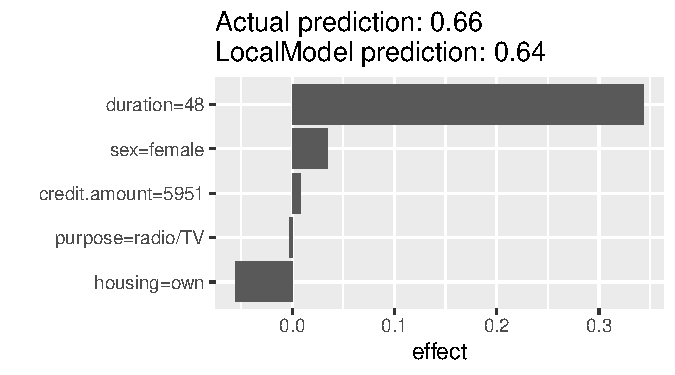
\includegraphics[width=0.45\textwidth]{figure/lime_credit.pdf}\\[-0.4em]
	Effects of surrogate model, i.e. $w^\top x$.
\end{center}

\end{frame}
%------------------------------------------------------
\begin{frame}{Credit Dataset}

\vspace{-2em}
\begin{itemize}
	\item The local model prediction for $x$ is $g(x) = 0.64$. 
	\item $g$ has a local fidelity of $L(\hat{f}, g, n) = 4.82$ with $n(z)$ as the Gower proximity and $L(\hat{f}_{bad}(z), g(z))$ as the euclidean distance. 
	\item 2-dim ICE plots (also called surface plot) of credit amount and duration show us how the surrogate model $g$ linearly approximates the previously nonlinear prediction surface of $\hat{f}_{bad}$. 
\end{itemize}
\vspace{-2em}
 \begin{columns}
	\begin{column}{0.35\textwidth}
		\begin{center}
		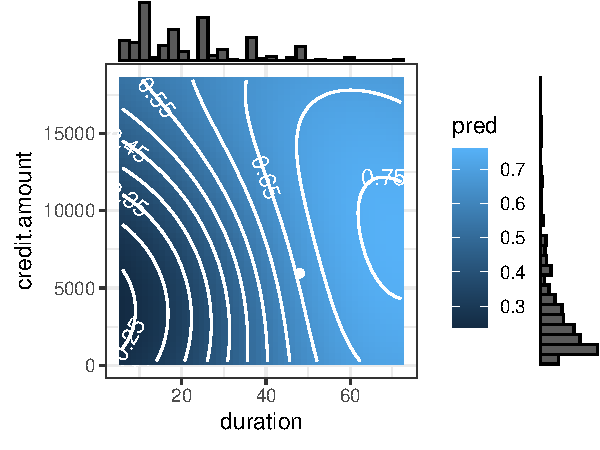
\includegraphics[width=1\textwidth]{figure/lime_credit_ice1.pdf}
		\end{center}		
	\end{column}
	\begin{column}{0.35\textwidth}  
		\begin{center}
				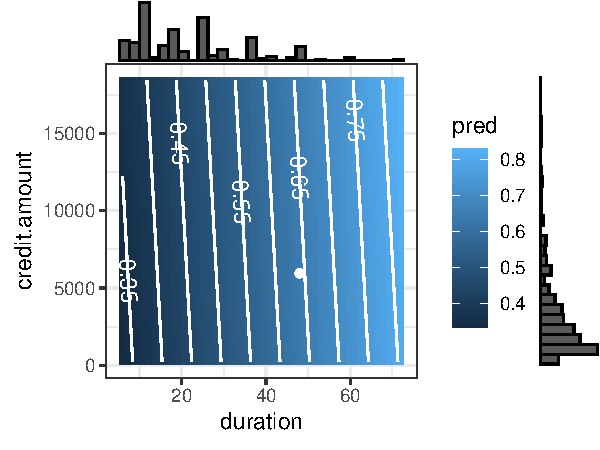
\includegraphics[width=1\textwidth]{figure/lime_credit_ice2.pdf}
		\end{center}
			
	\end{column}
\end{columns}
\begin{center}
    real model $\hat{f}$ vs. surrogate $g$
\end{center}
%\vspace{-0.4cm}
% \begin{center}
% 		\tiny{\textbf{Figures:} 2-dim ICE plot of $\pih_{bad}$ (\textbf{left}) and surrogate $g$ (\textbf{right}) for features duration and credit amount. \\The white dot is $x$. The histograms display the marginal distribution of the training data $\Xmat$.}
% \end{center}

\end{frame}

%\begin{frame}{Bike Sharing Dataset}
%\vspace{-.3cm}
%
%\begin{center}
%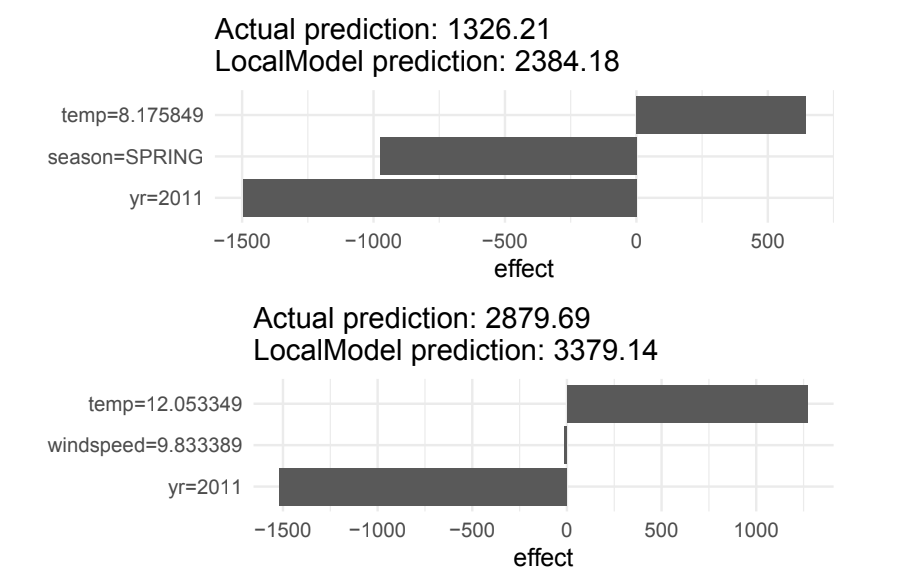
\includegraphics[width=0.7\textwidth]{figure/bike-figure.png}
%\end{center} 
%
%\footnotesize \textbf{Figure:} LIME for two example instances of the bike sharing dataset.
%
%\normalsize
%\vspace{0.2cm}
%The plots show the feature effect of the sparse linear model, i.e. the model coefficients times the feature value of the instance.
%Warmer temperature has a positive effect on the prediction, 
%while the year 2011 has a large negative effect as well as the springtime.
%\end{frame}

\begin{frame}[c]{LIME for Text Data \lit{Shen 2019}{https://medium.com/just-another-data-scientist/explain-sentiment-prediction-with-lime-f90ae83da2da}}
	\begin{itemize}
		\item Raw text as a data frame by transforming it into a binary vector (e.g., a vector of word counts).
		\item texts \textit{``This text is the first text."} and \textit{``Finally, this is the last one."}:
		\begin{center}
			\begin{tabular}{c|c|c|c|c|c|c|c} 
				this & text & is & the & first & finally & last & one \\ 
				\hline
				1 & 2 & 1 & 1 & 1 & 0 & 0 & 0 \\
				1 & 0 & 1 & 1 & 0 & 1 & 1 & 1 \\
			\end{tabular}
		\end{center} 
		\item New samples $z$ by randomly setting the entry of individual words to $0$\\ i.e. equal to removing all occurrences of this word in the text. 
		\item An exponential kernel with cosine distance as a proximity measure. 
		\item Cosine distance is advantageous  because it neglects words not occurring in both texts and measures the distance irrespective of the text size. 
	\end{itemize}

\end{frame}

\begin{frame}[c]{LIME for Text Data \lit{Shen 2019}{https://medium.com/just-another-data-scientist/explain-sentiment-prediction-with-lime-f90ae83da2da}}

    \begin{itemize}
		
		\item Below LIME explains a random forest classifier that labels movie reviews from IMDB. 
		\item The surrogate model is a sparse linear model. 
	\end{itemize}
	
	\begin{figure}
		\begin{center}
			%\captionsetup{font = scriptsize, labelfont = {bf, scriptsize}}
			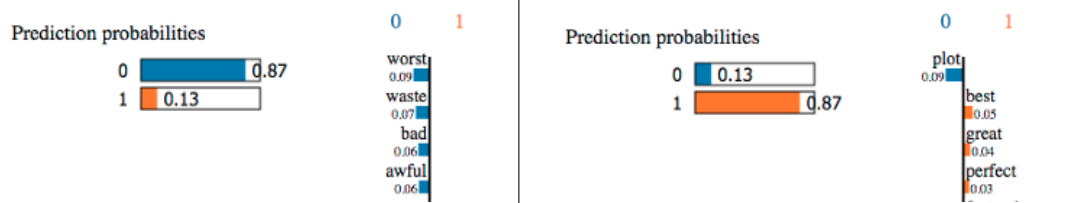
\includegraphics[width=0.9\textwidth]{figure/lime_movier}
		\end{center}
	\end{figure}
	
\end{frame}
	
\begin{frame}[c]{LIME for image data \lit{Achanta et al. 2012}{https://ieeexplore.ieee.org/document/6205760}}
	\begin{columns}
		\begin{column}{0.67\textwidth}
			\begin{itemize}
				\item Each instance is represented as a binary vector indicating the presence or absence of superpixels. 
				\item Superpixels are interconnected pixels with similar colors. They are used because a single pixel would probably not change a prediction by much.
				\item Challenge: The size of superpixels needs to be determined before the segmentation takes place.
				\item New samples $z$ are created by randomly switching some of the super pixels ``off", i.e., by coloring some superpixels uniformly.  
			\end{itemize}		
		\end{column}
		\begin{column}{0.26\textwidth}  
		
			\begin{center}
				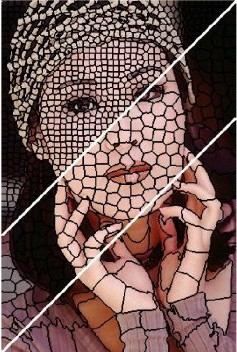
\includegraphics[width=.7\textwidth]{figure/superpixel_woman}\\
				 Example for superpixels of different sizes.
			\end{center}
			
		\end{column}
	\end{columns}
\end{frame}

\begin{frame}[c]{LIME for image data \lit{Ribeiro et al. 2016}{https://arxiv.org/abs/1602.04938}}
	\begin{itemize}
		\item Below, LIME explains the prediction of Google's pre-trained Inception neural network classifier of an arbitrary image. 
		\item Samples $z$ are created by graying out all superpixels besides 10. 
		\item As a surrogate model, locally weighted sparse linear models are trained to predict the probability of each class. 
		\item Weights are determined by an exponential kernel with euclidean distance.
		\item Below the corresponding explanations for the top 3 predicted classes are shown.   
	\end{itemize}
% https://lime-ml.readthedocs.io/en/latest/lime.html#module-lime.lime_image
	\begin{center}
		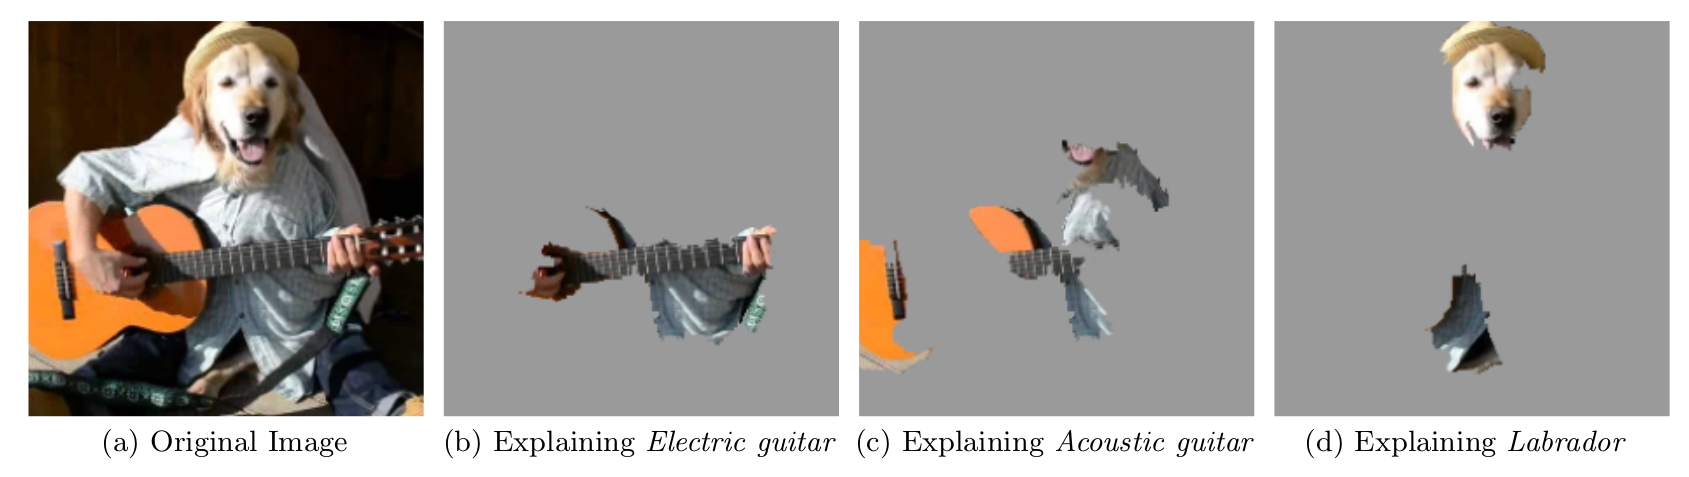
\includegraphics[width=0.7\textwidth]{figure/lime-images}
	\end{center}
\end{frame}

\begin{frame}{Anchors for Tabular Data: Bike Rental I \lit{T. Goerke \& M. Lang}{https://christophm.github.io/interpretable-ml-book/anchors.html}}
    \vspace{-2em}
    \begin{itemize}
        \item Task: Classify whether the number of rented bikes is above or below the average?
    \end{itemize}
    
    \centering
    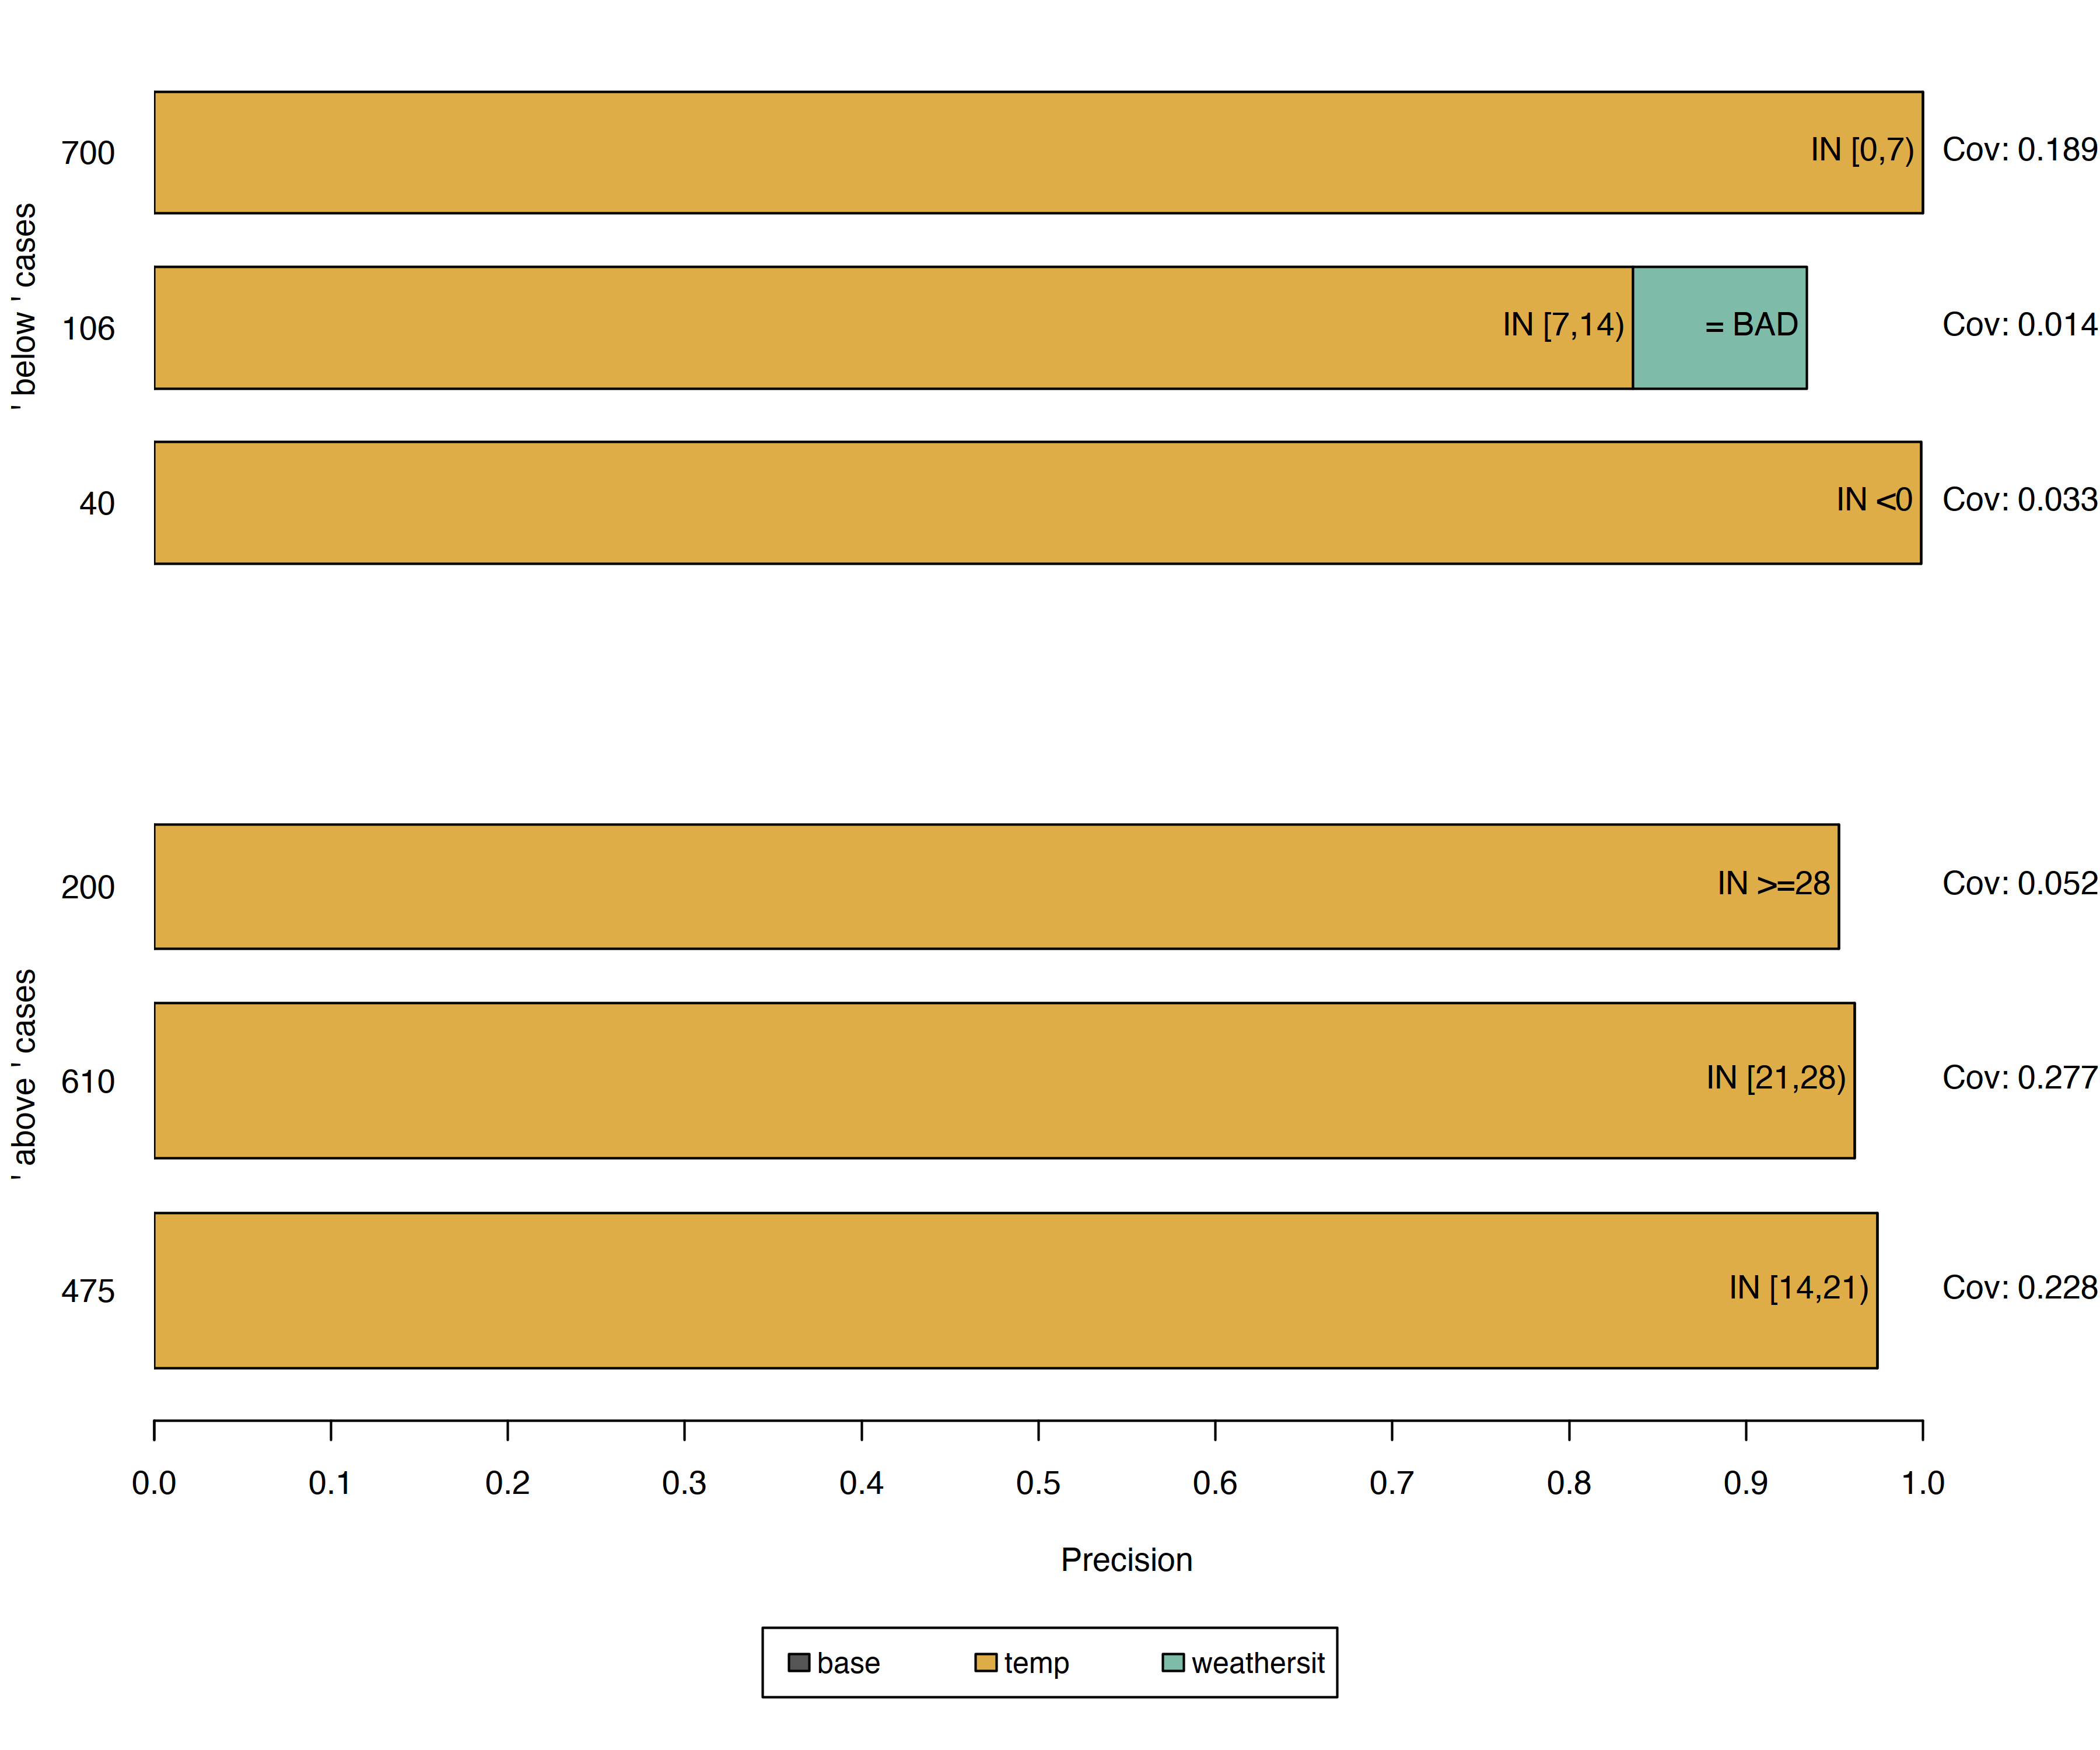
\includegraphics[width=0.6\textwidth]{w04_local_explanations/figure/bike_anchor1.png}
    
\end{frame}

\begin{frame}{Anchors for Tabular Data: Bike Rental II \lit{T. Goerke \& M. Lang}{https://christophm.github.io/interpretable-ml-book/anchors.html}}
    
    \vspace{-2em}
    \begin{itemize}
        \item Task: Classify whether the number of rented bikes is above or below the average?
    \end{itemize}
    
    \centering
    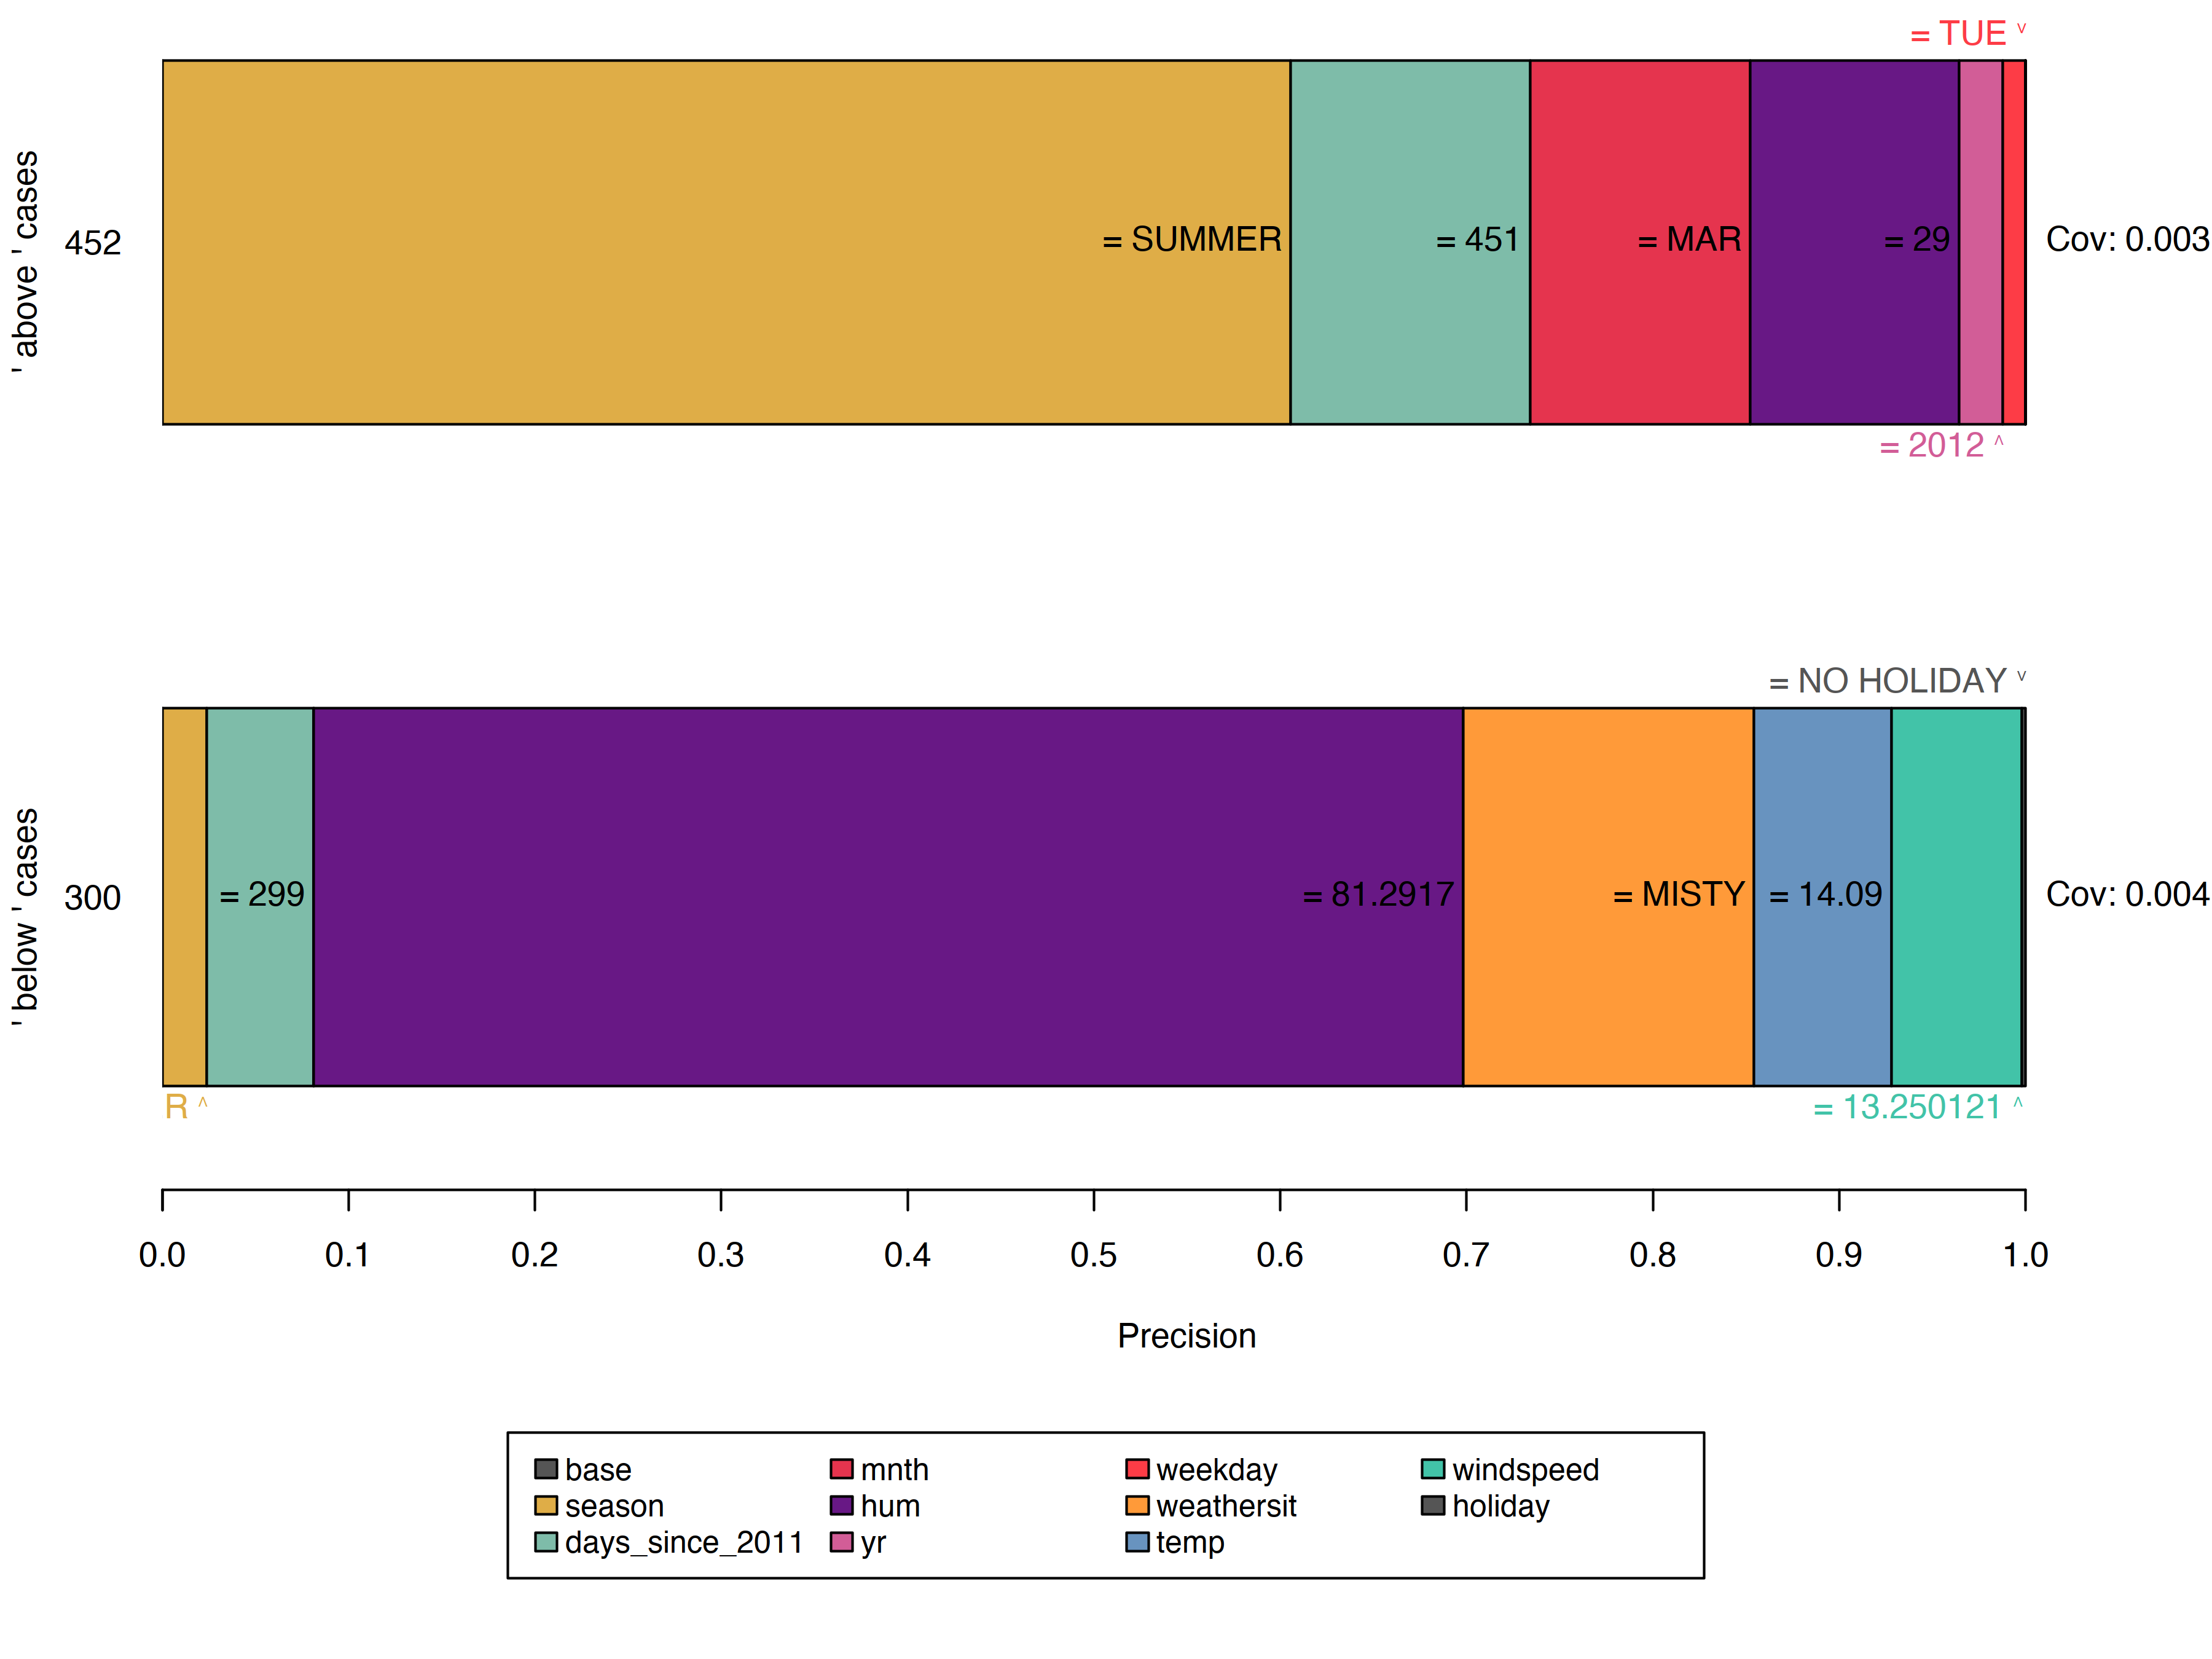
\includegraphics[width=0.62\textwidth]{w04_local_explanations/figure/bike_anchor2.png}
    
\end{frame}

% Counterfactuals Examples
% \begin{frame}[c]{Example CE: Credit Data}
% 	\begin{itemize}
% 		\item Model: SVM with RBF kernel
% 		\item $x$ is the first data point of the dataset with $P(y = good)  = 0.34$ of being a ``good" customer.  
% 		\item Our desired goal is to increase the probability to $[0.5, 1]$.
% 		\item Mulit-objective CE found 82 counterfactuals.
% 		\item All counterfactuals proposed changes to the credit duration and many to the credit amount.  
% 	\end{itemize}
	
% \end{frame}
% \begin{frame}{Example CE: Credit Data}
%     \vspace{-2em}
% 	\begin{columns}
% 				\begin{column}{0.5\textwidth}  
% 			\begin{center}
% 				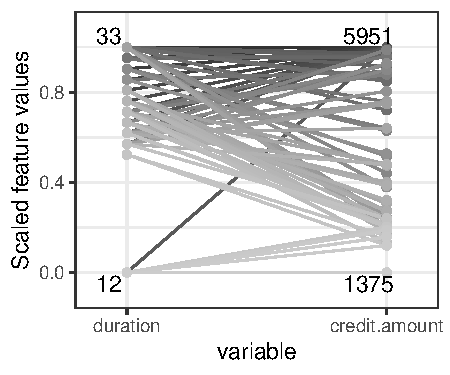
\includegraphics[width=0.6\textwidth]{figure/counterfactuals_credit_parallel}
% 			\end{center}
			
% 		\end{column}
% 		\begin{column}{0.5\textwidth}
% 			\begin{center}
% 				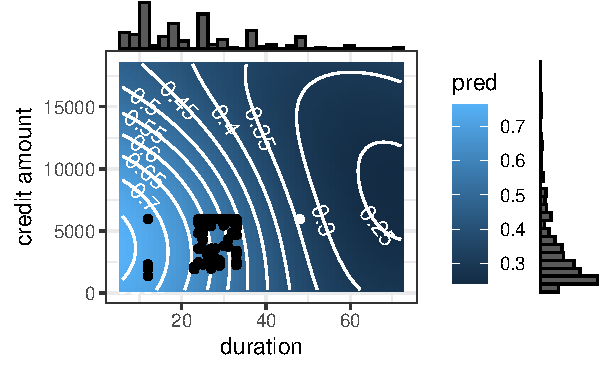
\includegraphics[width=.8\textwidth]{figure/counterfactuals_credit_heat}
% 			\end{center}
				
% 		\end{column}
% 	\end{columns}
	
% 	\begin{itemize}
% 	    \item Parallel plot (left): all counterfactuals had values equal to or smaller than the values of $x$.
% 		\item Surface plot (right): why these feature changes are recommended. 
% 		\item Counterfactuals in the lower left corner seem to be in a less favorable region far from $x$, but they are in high density areas close to training samples (indicated by histograms).
% 	\end{itemize}
		
% \end{frame}


\end{document}